\section{Arkitektur}\label{sec:arkitektur}
\als{Nu falder Dannebrog ned fra himlen igen}
Dette afsnit præsenterer arkitekturen som er udarbejdet på baggrund af de specificerede behov i \cref{arkitekturkrav}.
Først beskrives den overordnede opbygning.
Derefter beskrives komponenterne mere detaljeret.

\paragraph{Platform}
Android er blevet valgt som platform, se \cref{sec:valg_af_android}, hvilket også lægger op til nogle overvejelser ift. arkitektur.

Arkitekturen er lavet ud fra ideen om at applikationer på Android kan kontakte hinanden igennem Android systemet.
Det er muligt for en hovedapplikation at starte en service der ligger i en anden applikation \citep{android_service}.\lars{herfra}
Dette udnyttes ved at pakke alle moduler i hver deres selvstændige applikation.
Ved at anvende en centraliseret database vil det være muligt for moduler at få adgang til data fra andre moduler.
Samtidig kan adgangsrettigheder til de forskellige tabeller styres et sted.
På den måde kan adgang kontrolleres på alle moduler, inklusiv de der måtte blive udviklet i fremtiden.
Hertil ønskes en central styrende enhed, der skal fungere som bindeled mellem de installerede moduler.
\lars{ og hertil tror jeg ikke bør nævnes, da det sådanset er hvad den næste section indeholder}

\subsection{Opbygning}\label{arkitektur:opbygning}
Den overordnede arkitektur er opbygget af fire komponenter: \textit{manager}, \textit{moduler}, \textit{DB\footnote{Database} access} og \textit{DB}.
For at opfylde de specificerede behov i \cref{arkitekturkrav}, nærmere nøgleordene \textit{modulær}(se \cref{arkitekturkrav::modulaer}) og \textit{fleksibel}(se \cref{arkitekturkrav::fleksibel}) er arkitekturen opbygget af moduler der opsamler data, analyserer data og viser det uafhængigt af hinanden.
Disse moduler kan vælges til eller fra i \textit{manager}'en.


Et diagram over arkitekturen kan ses på \cref{arkitektur_udkast_1}.
\begin{figure}[h]
	\centering						%  l   b   r	t
	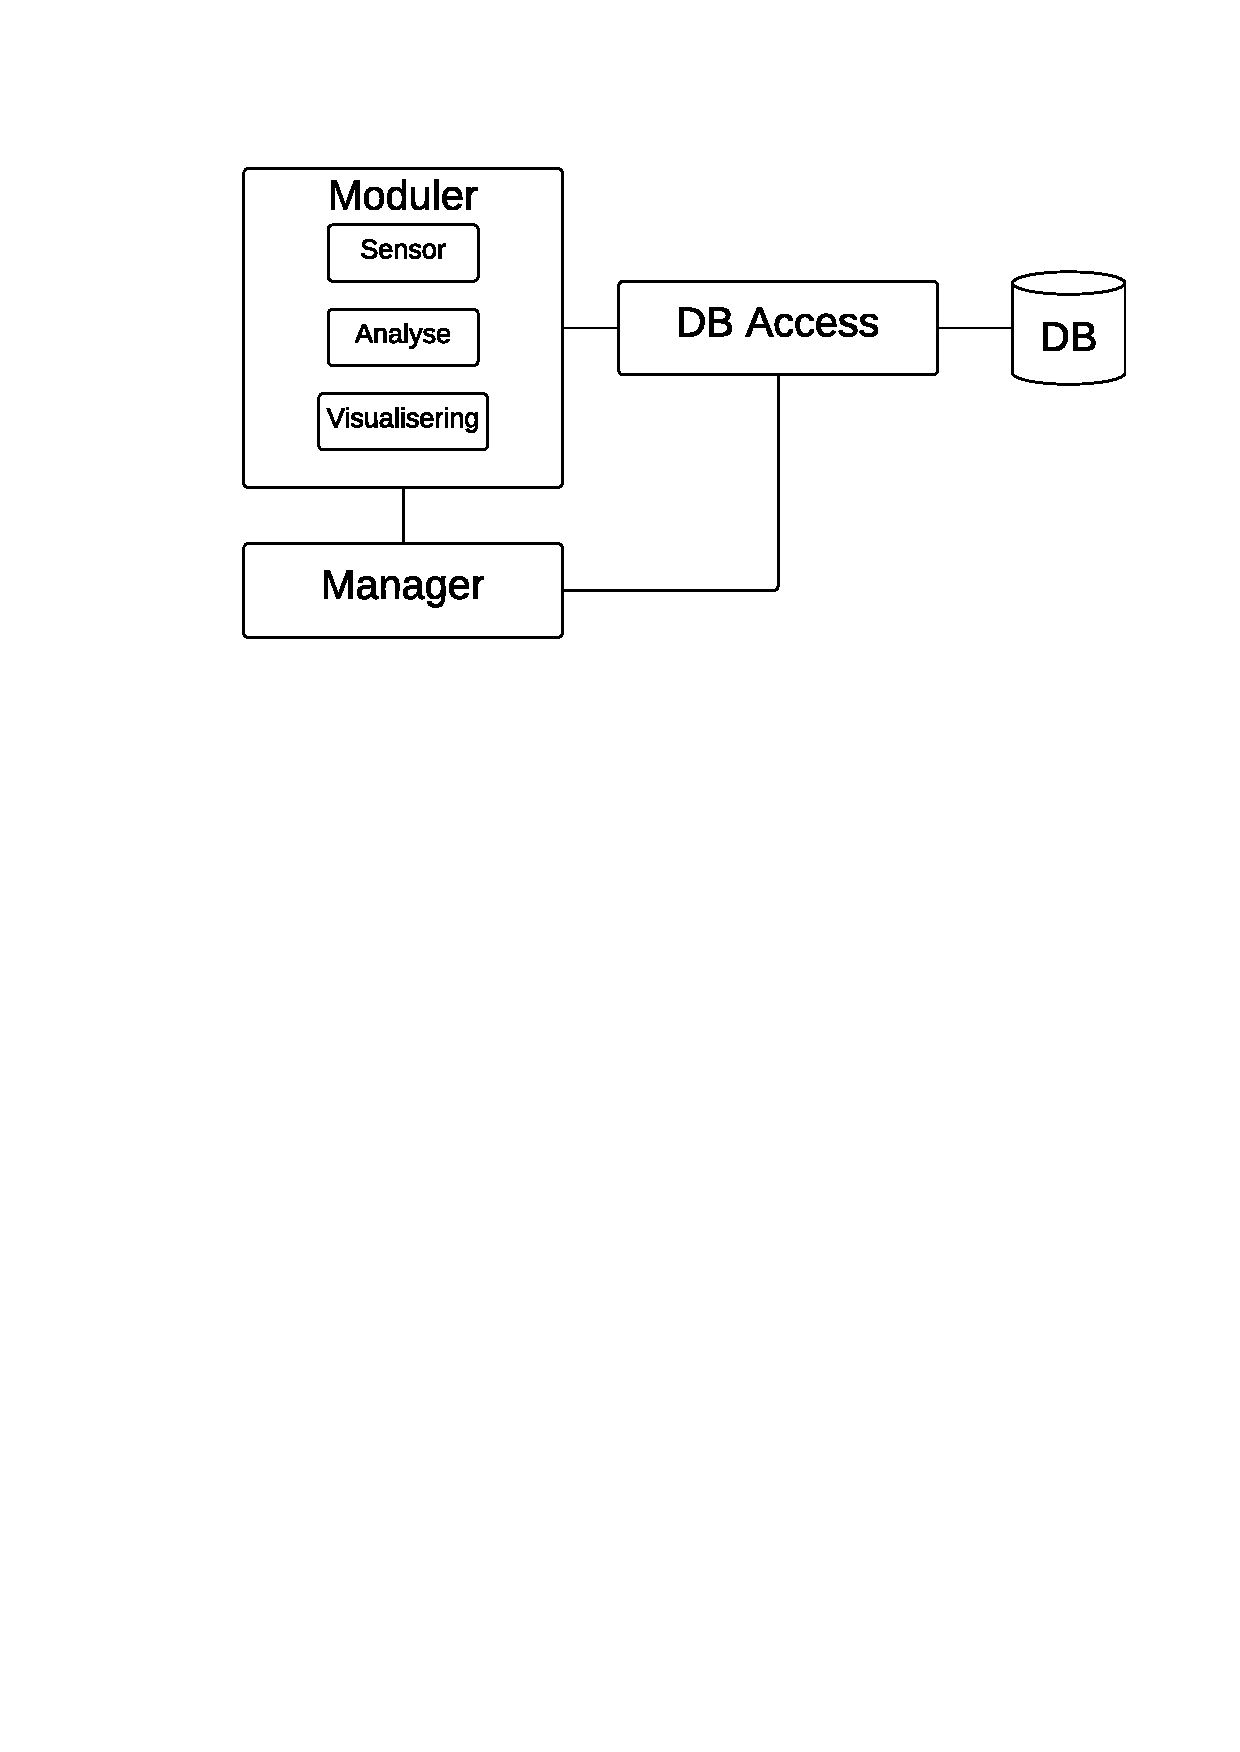
\includegraphics[scale=0.5, trim = 1cm 17.5cm 1cm 1cm, clip]{ArkitekturLucidChart}
	\caption{Systemets arkitektur}
  \label{arkitektur_udkast_1}
\end{figure}

\lasse{Ivan vil have noget med patterns her, men troede vi fjernede det?}

Herefter beskrives komponenterne i rækkefølge af deres indbyrdes afhængighed, således at forståelsen af hver komponent kun afhænger af det læste.

\subsection{DB}
Denne komponent administrerer data for systemets forskellige moduler.
Data opbevares i en række tabeller i et relationelt database system.
Hvert modul har mulighed for at definere egne tabeller, der alle gemmes i \textit{DB} komponenten.

Til dette projekt er der valgt en SQLite database da denne er standard i Android \citep{android_database}.


\subsection{DBAccess}\label{subsec:DBACCESS}
Denne komponent styrer adgangen til \textit{DB} komponenten så det sker på en ensrettet måde.
Da vi arbejder på en mobil platform er det værd at tage højde for lagerstyring og abstraktion derover.
Da der er begrænset plads på en smartphone kan det blive relevant at lagre noget af det indsamlede data i skyen.
Grundet denne potentielle opdeling af hvor data er lagret, kan det være nyttigt at abstrahere over hvor data er lagret.\lasse{Han forstår ikke abstrahere. Jeg kunne ikke beskrive det ordentligt.}

For at opfylde nøglepunktet \textit{kommunikativ}, se \cref{arkitekturkrav::kommunikation}, er det nødvendigt at sørge for at moduler har adgang til kun at skrive til deres egen database og samtidig læse fra alle andres database.
På denne måde forhindres det at eksterne moduler modificerer andre modulers data.
Dette er dog ikke blevet implementeret, men bliver diskuteret yderligere i \cref{databaserettigheder}.

\paragraph{Design} 
DB access benytter implementerer en \textit{ContentProvider} \citep{contentprovider}, der er et interface som Android stiller tilrådighed.
Content Providers er en måde hvorpå man kan stille data til rådighed for andre apps i Android.

Brugen af content provideren gør også at interfacet til DB access er veldefineret.
Ændring af lagringsmetoden eller tilføjelsen af backup i skyen vil kunne gøres under dette interface, så det ikke ødelægger kompatibilitet til moduler.

\subsection{Moduler}
Denne komponent befinder sig i et lag for sig selv og indeholder tre typer moduler: \textit{data}, \textit{analyse} og \textit{visualisering}.
Modulkomponenten indeholder applikationens hovedfunktionalitet og er ansvarlig for indsamling af data, bearbejdelse af data og visualisering af data.

Dette afsnit beskriver hvordan modulerne er defineret og giver en beskrivelse af de tre typer moduler.
Men først følger en begrundelse for valget af dette lag på baggrund af behovene i \cref{arkitekturkrav}.

\paragraph{Begrundelse for valg}
For at opfylde nøgleordet \textit{modulær}(se \cref{arkitekturkrav::modulaer}) er det valgt lave et lag der indeholder moduler, så det er let at tilføje og fjerne moduler.
Dette kunne fx være i en situation hvor der kommer nye sensorer på markedet, eller hvis der skal laves nye former for visualiseringer til det allerede indsamlede data.
Desuden opfylder det også nøgleordet \textit{kombinerbar}, fordi fx moduler fra \textit{data} kan kombineres til at lave et \textit{analyse}-modul.

%Måde at lave eksterne modul-applikationer uden at ændre hoved-applikation.
%Definere output (tabeller/kolonner), samt input (afhængigheder)
%Evt. konfigurationsmuligheder for moduler afhængige af det
%Fleksibel måde at modtage data fra andre moduler, uden at skulle opdatere applikation(erne). Dvs. ikke design-mønstre: observer, mediator, men gennem content provider.
% modularisering i Android; multiple applikationer under samme package

For at opfylde kravet om fleksibilitet der er stillet til systemet, har vi udtænkt en modulbaseret arkitektur der gør det let at tilføje moduler til pakken.
Det skal være muligt at tilføje eksterne moduler, uden at have behov for at lave ændringer i hoved-applikationen.
Dette kan gøre sig gældende når der kommer nye sensorer på markedet, eller hvis der skal laves nye former for visualiseringer til det allerede indsamlede data.
\subsubsection{Forslag til modulariseing}
\paragraph{Komplet Pakke}
En traditionel applikation samler al funktionalitet i en pakke.
Hvis man udvikler på dele af applikationen vil en opdatering skulle ske af hele appen på samme tid.
Desuden bliver det sværere for eksterne udviklere at bidrage til applikationen, da opdateringer skal ske igennem udviklerne af hovedapplikationen.

\paragraph{Import af Kode}
En anden mulighed er at inkludere et scripting sprog med applikationen og gøre det muligt at udvikle script der kan agere modul.
Denne løsning kræver et meget kraftigt scripting sprog hvis alle Androids muligheder skal stilles til rådighed.
Hvis scripts på den anden side skal skrives direkte i java vil der være nogle sikkerhedshensyn som vil gøre det svært at kontrollere hvad moduler kan og ikke kan.
For eksempel vil det være vanskeligt at kontrollere hvilke database tabeller der er adgang til.
Sikkerhedsproblemet er stort, men kunne sikkert løses med nok tid og ressourcer.

\paragraph{Selvstændig Applikation}
Den tredje mulighed er at pakke hvert modul i en selvstændig APK \footnote{Androids pakkeformat}.
Denne APK skal indeholde en beskrivelsesfil som læses i hoved-applikationen og indeholder information om modulet.
Denne metode sørger for at hoved applikationen kan kontrollere hvad moduler har adgang til. 

Ulemper ved denne løsning er at den er knap så lightweight, idét at det kræver at en stor mængde af applikationer skal installeres.
Derudover er kommunikation mellem applikationer vanskeligere end internt i en applikation, men ses som acceptabelt.
Desuden kan det være træls at skulle installere en større mængde af applikationer for at have den fornødne funktionalitet.
Som løsning derpå kunne man med videre arbejde have et indbygget applikation marked i manageren, og er værd at udforske med mere tid.

Det er en løsning der har mange fordele i forhold til modularisering og svagheder der kan tolereres, hvorfor denne løsning er valgt. 

Det følgende vil forklare detaljerne i implementationen af moduler ved hjælp af selvstændige applikationer.

\subsubsection{Beskrivelsesfilen}

Til dette er der valgt at bruge JavaScript Object Notation (JSON) samt JSON Skema \citep{jsonpojo}.
Eksemplerne der bruges herefter vil derfor være i henholdsvis JSON eller JSON Skema.

\subsubsection{Typer af Moduler}
Der findes som sagt i \cref{sec:arkitektur}, tre typer moduler: \textit{sensor}, \textit{analyse} og \textit{visualisering}.
Som sagt er sensor moduler, moduler som indsamler data fra telefonens forskellige sensorer og applikationer.
Endvidere er analyse moduler, moduler som bruger data fra enten sensor eller andre analyse moduler til at bearbejde data med den hensigt at opnå en opsummering af data som kan videre bruges af systemet til enten visualisering eller videre bearbejdning.
Visualiseringsmodulerne bruges til visualisering af den rå sensor-data eller den behandlede analyse-data.

\subsubsection{Moduldefinition}
Som minimum har et modul et navn og en version, så andre moduler kan referere dem.

Sensor- og analyse-moduler skal gøre data tilgængeligt for andre analyse- og visualiserings-moduler.
For at specificere hvordan data skal gemmes, samt hvad der er tilgængeligt for andre, skal dette defineres for hvert modul af førstnævnte typer.
For hvert modul skal der defineres en eller flere tabeller som modulet kan gemme data i.
For hver tabel defineres en eller flere kolonner med et beskrivende navn, datatype og evt. en måleenhed.

\subsubsection{Data Typer}
De tilgængelige data typer tilgængelig for tabel-kolonner, er begrænset til de tilgængelige SQLite datatyper.
Der er 5 typer: \textit{NULL}, \textit{INTEGER}, \textit{REAL}, \textit{TEXT} og \textit{BLOB}.

\subsubsection{Afhængigheder}
Et analyse- eller visualiserings-modul kan være afhængigt af andre sensor- eller visualiserings-moduler.
Et analysemodul kan aggregere data fra andre analysemoduler mens et visualiseringsmodul er afhængig af det modul det skal vise data fra.
Derfor skal det defineres for hvert modul hvilke andre moduler det er afhængigt af.
Der findes to grader af afhængigheder i systemet: hard- eller soft-dependency.
En hard-dependency er ét andet modul som det pågældende modul ikke kan fungere uden.
En soft-dependency er en liste af andre moduler, hvor mindst ét af de listede moduler skal være til stede på enheden.
Dette er nyttigt hvis et modul skal bruge eksempelvis accelerometer data, men det er ikke vigtigt om det kommer fra en telefon eller fra en wearable.

\subsubsection{JSON og JSON Schema}
For at have en modul-beskrivelse der er læselig for både mennesker og maskiner, er JSON valgt.
JSON gør det muligt for ikke-tekniske personer at læse, skrive og forstå definitionen af et modul.
For at sikre validiteten af eksternt leverede modul-beskrivelser, udarbejdes der et JSON Skema, som JSON-dokumenter kan holdes op imod og derved verificeres.
Det anvendte JSON Skema kan findes i \cref{app:json_schema}.

\paragraph{Eksempel} på en modul-beskrivelse.
Meta-data er præfikset med \_ (underscore).
\begin{lstlisting}
{
  "name": "accelerometer",
  "_version": 1.0,
  "tables": [
    { "name": "accelerations",
      "columns": [
        { "name": "accX",
          "dataType": "REAL",
          "_unit": "g" },
        { "name": "accY",
          "dataType": "REAL",
          "_unit": "g" },
        { "name": "accZ",
          "dataType": "REAL",
          "_unit": "g" }
      ]}]}
\end{lstlisting}

\subsubsection{Implementering}
Som nævnt i \cref{sec:valg_af_android}, implementeres der til Android telefoner.
Dette sætter nogle begrænsninger ift. valg af løsninger.

\subsubsection{JSON kontra XML}
XML ville være det naturlige valg for Android applikationer, da en del af applikations udvikling foregår i XML fordi man ofte bruger det til at definere layouts og definering af statiske ressourcer. 
Dog blev JSON valgt over XML, da vi gerne ville have automatisk generering af en parser ud fra skemaet.
En automatisk genereret parser vil lette arbejdet med et skema der i udviklingsperioden ændres ofte.
Denne automatiske generering viste sig ikke at være ligetil på grund af kompatibilitetsproblemer på Android, mens det var enkelt at udføre i JSON.

\subsubsection{Moduler som Applikationer}
For at det skal være muligt at installere moduler uden at opdatere hoved-applikationen, skal der installeres applikationer via Google Play Store.
Alle modul-applikationer, samt hoved-applikationen, deler \textit{package}-navn.
Hver modul-applikation har sin JSON beskrivelse som en eksternt tilgængelig \textit{ressource}, som hoved-applikationen eller andre moduler har adgang til.
Kommunikation mellem applikationer foregår med \textit{services}, \textit{intents} eller \textit{content provider}.

\subsubsection{Håndtering i Manager}
Håndteringen af moduler sker i manageren, beskrevet i \cref{subsec:arkitektur-Manager}.
Når der tilføjes eller opdateres et modul detekterer manageren dette ved at finde alle applikationer der er installeret under pakken ``dk.aau.cs.psylog''.
Manageren læser alle moduldefinitioner efter at have valideret dem op imod JSON skemaet.
Alle moduler der har opdateret versionsnummer eller er helt nye vil blive håndteret ved at manageren læser tabelinformation ind fra moduldefinitionen og opretter eller ændrer de pågældende tabeller.

Når modulernes tabeller er blevet oprettet bygges en graf over afhængigheder, som bruges til at vise brugeren hvilke moduler der kan aktiveres.
Denne proces er yderligere beskrevet i \cref{sec:settings}


\subsection{Manager}\label{subsec:arkitektur-Manager}
Dette afsnit begrunder valget af denne komponent.
Derefter beskrives komponenten.

\paragraph{Begrundelse for valg}
For at opfylde nøgleordet \textit{fleksibel}(\cref{arkitekturkrav::fleksibel}), er der tilføjet en komponent kaldet manager.
Manager komponenten kan siges at være grænsefladen mellem bruger og moduler.
Den står for at administrere de installerede moduler ud fra de beskrivelser der er givet for de enkelte moduler.
Denne administration indebærer blandt andet oprettelse af de database tabeller hvert modul har bedt om i sin beskrivelse, samt start og stop af sensor- og analysemoduler.
Sidstnævnte sker ud fra definitioner givet i beskrivelserne af de enkelte moduler.
Desuden er det også gennem manageren at brugeren får vist information, såsom visualiseringer.

\subsubsection{Beskrivelse af manageren}
Manageren er den eneste komponent brugeren interagerer med.
Det er igennem manageren at brugeren vælger hvilke moduler der skal køre.
Det er også den der sørger for at de rigtige moduler kører på de rigtige tidspunkter.
Dette gøres ved hjælp af \texttt{TaskRunner}.
Derudover er det også manageren der sørger for at skaffe moduldefinitionen fra alle de installerede moduler.
Ydermere, giver manageren et overblik over de visualiseringsmoduler der er installeret samt have en måde at vise visualiseringsmodulerne på.
\paragraph{Udførsel af moduler}
Der er overordnet to måder hvorpå moduler køres; enten styrer de selv deres kørsel (kontinuerte kørende moduler) ellers administreres de af managerens \texttt{TaskRunner}, som er en \texttt{Service} der startes når mobilen tændes.
Både sensor- og analyse-moduler kan køre på disse to forskellige måder.

\subparagraph{Kontinuerligt kørende moduler}
Til moduler der skal køres kontinuert, startes deres \texttt{Service} så snart modulet aktiveres i indstillinger, hvorefter det selv administrerer hvornår og hvor ofte det udfører sin opgave.
Dette er for moduler der skal samle kontinuert data ind, som fx et modul der bruger accelerometer.

\subparagraph{TaskRunner}
Derudover er der også moduler, som kun skal køres på faste intervaller eller bestemte tidspunkter.
Her er der ikke behov for at det enkelte modul har en kontinuert kørende \texttt{Service}, idet Manageren starter modulets opgave på det korrekte tidspunkt.
På denne måde spares der ressourcer, da modulet kun aktiveres i den tid hvor det skal udføre sin opgave. 

Når \texttt{TaskRunner}en startes, danner den en liste over de moduler der skal køres med interval eller på fast tidspunkt.
Derefter laver den en prioriteret kø, sorteret efter næste kørsels-tidspunkt.
\texttt{TaskRunner} tråden venter så, indtil næste opgave skal udføres.
Efter opgaven er udført udregnes næste kørsels-tidspunkt for den netop kørte opgave, hvorefter prioritets-køen sorteres.
Så venter tråden igen, indtil næste kørsels-tidspunkt, og dette fortsætter så længe der er aktive moduler, som skal køres på denne måde.

\paragraph{Indstillinger}\label{sec:settings}
En af komponenter der skulle laves var en side der kan aktivere eller deaktivere moduler, det vil sige en indstillings side. Dette afsnit beskriver dette.

%guidelines
For at få en velkendt og standardiseret brugergrænseflade fulgtes android design guidelines.
Disse guidelines angiver hvornår man skal bruger diverse knapper, actionbars, settings etc.
\cite{androiddesign}

%Prototypes
Ved at følge disse guidelines blev en række prototyper for indstillinger lavet.
Disse byggede på samme princip om at udarbejde en indstillingsmenu.
Der var diskussion om hvordan disse skulle være, men over flere iterationer valgtes der at gå fra en ``wizard'' tilgang til en regulær settings menu,
Billeder af diverse prototyper kan ses i \cref{fig:prototype-manager}

\begin{figure}[H]
	\centering
	\begin{subfigure}[b]{0.45\textwidth}
			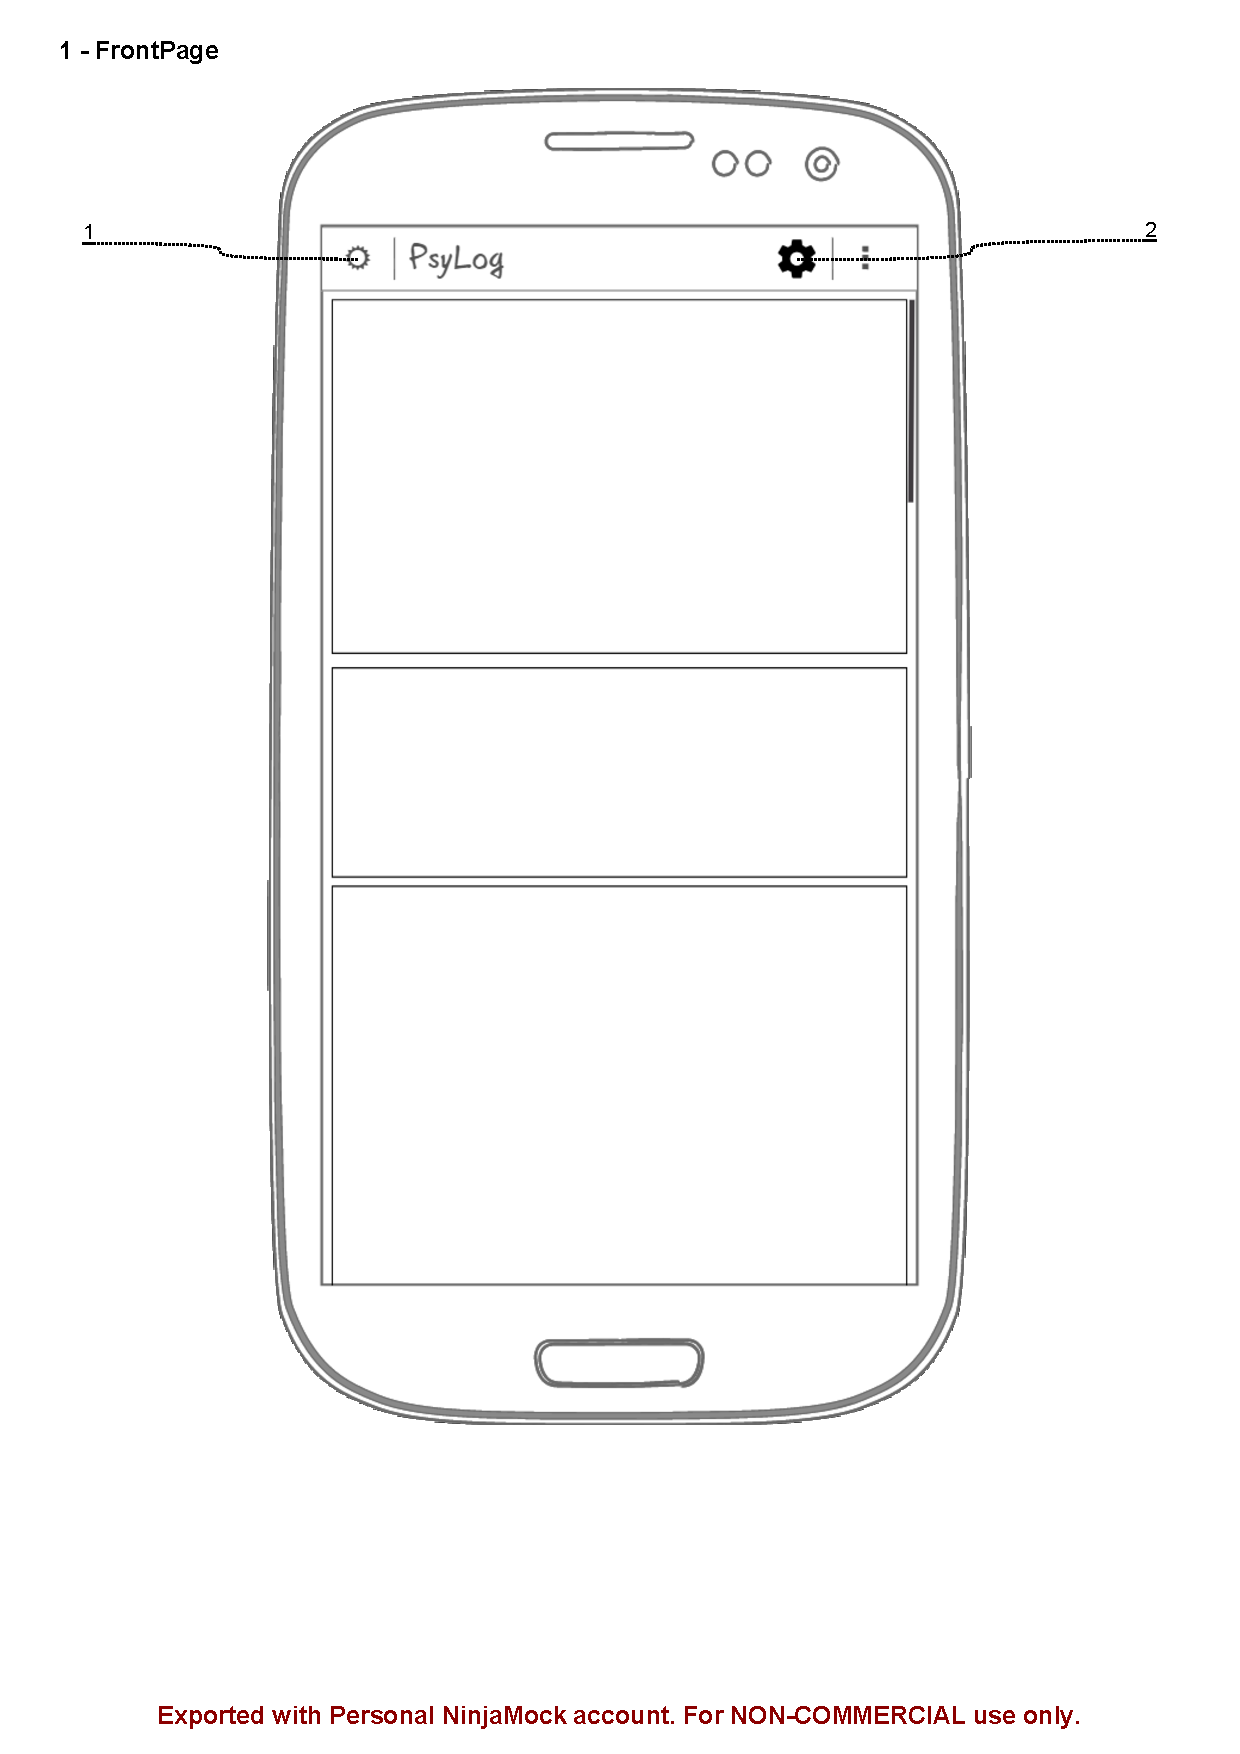
\includegraphics[scale=0.3, page=1, trim = 1cm 5.5cm 1cm 0cm, clip]{prototype.pdf}
			\caption{Forside}
	\end{subfigure}
	\begin{subfigure}[b]{0.45\textwidth}
			\includegraphics[scale=0.3, page=2, trim = 1cm 5.5cm 1cm 0cm, clip]{prototype.pdf}
			\caption{Indstillinger}
	\end{subfigure}
	\caption{Prototype af Manager}
	\label{fig:prototype-manager}
\end{figure}


%Actionbar
Ud fra prototypen kan en actionbar blandt andet ses, tanken er at følge et standard design hvor man har en actionbar i toppen.
Denne muliggør navigation til indstillinger, men også at gå tilbage til hovedmenuen, nuværende er der dog problemer med at den ikke vises under settings\als{Skal have lavet mere arbejde med den}

%Indstillinger, checkbox
Til at angive om et givent modul skal være aktiveret eller ej bruges checkboxes.
Dette skyldes at det er et simpelt ja/nej valg. 
Tanken er så at de moduler man har valgt er dem der kører på telefonen.

%indstillinger, dependencies og events
For at scanne mobilen for de moduler der er installeret bruges JSONParser der tager vare af dette. \als{referer til JSONParser}
Dette giver udslag i en række moduler der har afhængigheder af andre moduler og skal takles.
JSONParseren giver som resultat en liste af moduler. Disse scannes så igennem for at finde deres afhængigheder.
Disse afhængigheder bruges så til at konstruere events (OnChange) til at fortælle de moduler der skal have besked når et givent modul aktiveres/deaktiveres.
Ved at lave en sådan række er der implicit konstrueret en dependency graph.
Og som resultat af dette kan man forestille sig et hierarki hvor et modul på det lavest liggende niveau medfører en kæde af deaktiveringer af moduler der eksplicit og implicit afhænger af dette modul.
\stefan{så vidt jeg ved sker dette ikke længere på samme måde, Winde (eller en der vil sætte sig ind i koden) bør nok revidere dette afsnit}

%indstillinger, onPause start og stop sensorer
Efter afhængighederne er enkodet i programmet mangler der at takle hvordan sensorer skal startes og stoppes fra indstillingsmenuen.
Til at takle dette bruger vi den allerede udviklede ServiceHelper\als{referer til denne}.
Der vælges så at starte og stoppe de fornødne sensorer i onPause, da det typisk er når man forlader en indstillingsmenu at man gerne vil have at indstillingerne træder i kraft, og sikrer også at man ikke skal klikke på ekstra knapper for at indstillingerne træder i kraft.
\paragraph{JSON-Parser}\label{subsub:JSONparser}
JSON-parserens job er at finde JSON filen for hvert eneste modul installeret på smartphonen, hvorefter dette parses over i en klasse, og derefter autogeneres klasser ud fra JSON filen.
Måden dette er gjort på er ved brug af `jsonschema2pojo' \citep{jsonpojo}, der gør det muligt at få genereret klasserne som passer til JSON skemaerne, men også at få parset JSON filerne over i en klasse. 

